% !TEX root = ../discriminative_filtering.tex

\section{Preface}
This chapter presents what Prof. Harrison and I currently believe about the DKF. D. Brandman had many insights during the development process and was instrumental in implementing the DKF for human neural decoding.

\section{Introduction} \label{s:intro}
Consider a state space model for $Z_{1:T}:=Z_1,\dotsc,Z_T$ (latent states) and $X_{1:T}:=X_1,\dotsc,X_T$ (observations) represented as a Bayesian network:
\begin{equation} \label{f:graphical_model}
\begin{CD}
Z_1 @>>> \cdots @>>>  Z_{t-1} @>>> Z_t @>>> \cdots  @>>> Z_T \\
@VVV @.	@VVV @VVV @. @VVV \\
X_1  @. @. X_{t-1} @. X_t @. @. X_T
\end{CD}
\end{equation}
The conditional density of $Z_t$ given $X_{1:t}$ can be expressed recursively using the Chapman--Kolmogorov equation and Bayes' rule~\cite[see][for further details]{Che03}
\begin{subequations} \label{e:s2:BF}
\begin{gather} p(z_t|x_{1:t-1}) = \textstyle \int p(z_t|z_{t-1}) p(z_{t-1}|x_{1:t-1}) \; dz_{t-1} , \label{e:s2:BFa} \\
p(z_t|x_{1:t}) = \frac{p(x_t|z_t)p(z_t|x_{1:t-1})}{\int p(x_t|z_t) p(z_t|x_{1:t-1}) \; dz_t} , \label{e:s2:BFb}
\end{gather}  
\end{subequations}
where $p(z_0|x_{1:0})=p(z_0)$ and where the conditional densities $p(z_t|z_{t-1})$ and $p(x_t|z_t)$ are either specified \emph{a priori} or learned from training data prior to filtering. 
Computing or approximating \eqref{e:s2:BF} is often called {\em Bayesian filtering}. Bayesian filtering arises in a large number of applications, including global positioning systems, target tracking, computer vision, digital communications, and brain computer interfaces~\cite{Che03,Bro12,Bra17}. 

Exact solutions to \eqref{e:s2:BF} are only available in special cases, such as the Kalman filter~\cite{Kal60,Kal61}. The Kalman filter models the conditional densities $p(z_t|z_{t-1})$ and $p(x_t|z_t)$ as linear and Gaussian:
\begin{align} 
\label{e:s2:ZZ-1} p(z_t|z_{t-1}) & = \eta_d(z_t;Az_{t-1},\Gamma),  \\
\label{e:s2:KF-X} p(x_t|z_t) & = \eta_m(x_t;Hz_t,\Lambda),
\end{align}
so that the posterior distribution $p(z_t|x_{1:t})$ is also Gaussian and quickly computable. \textcite{Ben81} and \textcite{Dau84,Dau86} broadened the class of models for which for which the integrals in \eqref{e:s2:BF} are analytically tractable, but many model specifications still fall outside this class.  When the latent state space is finite, the integrals in \eqref{e:s2:BF} become sums that can be calculated exactly using a grid-based filter~\cite{Ell94,Aru02}.

For more general models, variational techniques have been developed that find a closely-related tractable model and use it to approximate the integrals in \eqref{e:s2:BF}.  For example, the extended Kalman filter (EKF) and the statistically-linearized filter fit a generic model to a linear model that then integrates exactly~\cite{Gel74,Sar13}.  Laplace and saddle-point approximations fit a Gaussian to an integrand by matching the local curvature at the maximum~\cite{But07,Koy10, Qua15}.  It is also possible to use Taylor series expansions, Fourier--Hermite series, or splines~\cite{Sar12}.  One issue with these approaches is that the approximating tractable models must be calculated online.  The EKF requires a derivative to be evaluated and tends to be quite fast, but methods such as the iterated EKF~\cite{Fri66,Wis69} and the Laplace transform entail solving an optimization problem in order to compute each filter update~\cite{Bel93}.  

Alternatively, a form for the posterior can be specified, and at each recursive update, the posterior can be approximated by a density closest to the required form.  This is known as the Assumed Density Filter~\cite{Kus67,Min01b}.  For example, when the specified form is Gaussian and the approximating density is chosen to minimize the KL-divergence between the true and approximate densities, the resulting filter estimates the posterior as a Gaussian having the same mean and variance as the calculated posterior~\cite{Sar13}.  For general models, we note that this still entails integration to calculate those first two moments.  Expectation Propagation extends Assumed Density Filtering with iterative refinement of estimates, but iterating over the entire history of observations is typically not practical in an online setting~\cite{Min01,Min01b}.

Solving the integrals in~\eqref{e:s2:BF} can be done using quadrature rules.  A primary example here are sigma-point filters including the unscented Kalman filter~\cite{Jul97,Wan00,van04}, Quadrature Kalman filter~\cite{Ito00,Ito00b} and  Cubature Kalman filter~\cite{Ara07,Ara09}.  Under these models, integrals are approximated based on function evaluations at deterministic points.

The integrals can also be solved using Monte Carlo integration~\cite{Met49}. Such approaches are called sequential Monte Carlo or particle filtering and include Sequential Importance Sampling and Sequential Importance Resampling~\cite{Han69,Han70,Gor93,Kit96,del96,Dou00,Cap05,Cap07}.    These methods apply to all classes of models but tend to be the most expensive to compute online and suffer from the curse of dimensionality~\cite{Dau03}.  Alternate sampling strategies~\cite[see, e.g.,][]{Che03,Liu08} can be used to improve filter performance, including: acceptance-rejection sampling~\cite{Han69}, stratified sampling~\cite{Dou05}, hybrid MC~\cite{Cho01}, and quasi-MC~\cite{Ger15}.  There are also ensemble versions of the Kalman filter that are used to propagate the covariance matrix in high dimensions including the ensemble Kalman filter~\cite[enKF:][]{Gei94} and ensemble transform Kalman filter~\cite[ETKF:][]{Bis01,Maj02}, along with versions that produce local approximations for covariance and can be parallelized~\cite{Ott02,Ott04,Hun07}.

In this paper we introduce another type of Gaussian approximation for \eqref{e:s2:BF}, called the {\em Discriminative Kalman Filter (DKF)}, that retains much of the computational simplicity of the Kalman filter, but that can perform well in several situations where existing approaches either fail or are too computationally demanding.  In particular, calculating an update step for the DKF entails only function evaluation and matrix algebra: neither optimization nor integration is required while the filter is online.

The DKF retains the linear, Gaussian model for the state dynamics $p(z_t|z_{t-1})$, but uses a discriminative formulation $p(z_t|x_t)$ for incorporating new observations instead of the generative specification $p(x_t|z_t)$.  Approximating $p(z_t|x_t)$ as Gaussian leads to a new filtering algorithm that can perform well even on models where $p(x_t|z_t)$ is highly nonlinear and/or non-Gaussian.  The model is Gaussian, but in a fundamentally different way, and it is allowed to be nonlinear, i.e.,
\begin{equation} 
\label{e:s2:DKF-X} p(z_t|x_t) = \eta_d(z_t;f(x_t),Q(x_t)) 
\end{equation}
where $f:\RR^m\to\RR^d$ and $Q:\RR^m\to\SS_d$, using $\SS_d$ to denote the set of $d\!\times\!d$ covariance matrices. There are several advantages to this approach:
\begin{itemize}
\item There is an exact, closed form solution for $p(z_t|x_{1:t})$ using \eqref{e:s2:BF} and the component densities specified in \eqref{e:s2:ZZ-1} and \eqref{e:s2:DKF-X}. This is true regardless of the functional form of the nonlinearities in $f(\cdot)$ and $Q(\cdot)$. See section~\ref{s:dkf}.  Note that a Gaussian Assumed Density Filter (ADF) under general specifications still entails integration for its update steps~\cite{Ito00,Ito00b}.
\item The Gaussian assumption in \eqref{e:s2:DKF-X}, which relates to the states, is often much more natural than the one in \eqref{e:s2:KF-X}, which relates to the observations. This is particularly true when $m\gg d$.  Under mild regularity assumptions, the Bernstein-von Mises Theorem states that $p(z_t|x_t)$ in equation \eqref{e:s2:DKF-X} is asymptotically normal (in total variation distance) as the dimensionality of $x_t$ increases. The observations themselves are not required to be conditionally Gaussian or even continuously-valued. For instance, in neural decoding, the observations are often counts of neural spiking events (action potentials), which might be restricted to small integers, or even binary-valued.
\item The DKF subsumes the Kalman filter as a special case by restricting $f$ to be linear and $Q$ to be constant. 
\end{itemize}

The DKF requires knowledge of the conditional mean and covariance of the latent state $Z_t$ given the observations $X_t$.  In some cases this information can be derived or approximated from a known model. If the observation model is unknown and must be learned from supervised training data prior to filtering (as is the case for our motivating BCI application) then it can be advantageous to learn these conditional means and covariances directly using off-the-shelf nonlinear and/or nonparametric regression tools, thereby avoiding some of the challenges of nonparametric density estimation.

%%%%%%%%%%%%%%%%%%%%%%%%%%%%%%%%%%%%%%%%%%%%%%%%%
\begin{figure}[h]
\begin{minipage}[t]{.45\textwidth}
\resizebox{0.6\textwidth}{!}{
$\begin{CD}
Z_{t-1}|X_{1:t-1} @>\eta_d(z_t;Az_{t-1},\Gamma)>>  Z_t \\
@.	@VV\eta_n(x_t;Hz_t,\Lambda)V  \\
@. X_t 
\end{CD}$
}
\end{minipage}%
\hfill
\begin{minipage}[t]{.45\textwidth}
\resizebox{0.6\textwidth}{!}{
$\begin{CD}
Z_{t-1}|X_{1:t-1} @>\eta_d(z_t;Az_{t-1},\Gamma)>>  Z_t \\
@.	@VV\approx\tfrac{\eta_d(z_t;f(x_t),Q(x_t))}{\eta_d(z_t;0,S)}V  \\
@. X_t 
\end{CD}$
}
\end{minipage}
\caption[A side-by-side comparison of the Kalman and Discriminative Kalman Filtering approaches]{On the left, we have the Kalman filter that takes both the measurement and state models to be linear, Gaussian.  On the right, we have the DKF that approximates $p(x_t|z_t)$ using Bayes rule and a nonlinear Gaussian approximation for $p(z_t|x_t)$.  For both of these filters, if $Z_{t-1}|X_{1:t-1}$ is normally distributed, then $Z_t|X_{1:t}$ can also be computed as normal with a closed-form recursion.}
\end{figure}

\section{Motivating the DKF}

Our motivating application for the development of the DKF is neural decoding for closed-loop brain computer interfaces (BCIs). BCIs use neural information recorded from the brain for the voluntary control of external devices~\cite{Wol02, Hoc06, Bra17}. Intracortical BCI systems (iBCIs) have been shown to provide paralyzed users the ability to control computer cursors~\cite{Pan15, Jar15}, robotic arms~\cite{Hoc12}, and functional electrical stimulation systems~\cite{Bou16,Aji17} with their thoughts. State-of-the-art decoding approaches have been based on the Kalman filter~\cite{Pan17, Jar15, Gil15}, which learns a linear model between neural features (observed) and motor intention (latent). Motor intentions are inferred from training data as vectors from the instantaneous cursor position to the target position $Z_t$ ~\cite{Bra18}. 

The DKF is a natural choice for closed-loop neural decoding using iBCIs placed in the primary motor cortex for a few reasons. First, evidence suggests that neurons may have very complex behavior. Neurons in the motor cortex have been shown to encode direction of movement~\cite{Geo88}, velocity~\cite{Sch94}, acceleration~\cite{Pan11}, muscle activation~\cite{Lem08, Poh07}, proprioception~\cite{Ben14}, visual information related to the task~\cite{Rao14} and preparatory activity~\cite{Chu12}. In particular, iBCI-related recordings are highly complex and their relationship with user intention may be highly non-linear \cite{Var15}. Moving away from the linear constraints of the Kalman filter could potentially capture more of the inherent complexity of the signals, resulting in higher end-effector control for the user. 

Second, evidence suggests that the quality of control is directly related to the rate at which the decoding systems perform real-time decoding. Modern iBCI sytems update velocity estimates on the order of 20ms~\cite{Jar15} or even 1ms~\cite{Pan15}. Thus any filtering technique must be computationally feasible to implement for real-time use.

Third, over the past decades, new technologies have allowed neuroscientists to record simultaneously from increasingly large numbers of neurons. The dimensionality of observed brain signals has been growing exponentially~\cite{Ste11}. By contrast,  the dimensionality of the underlying device being controlled remains small, generally not exceeding ten dimensions~\cite{Wod15,Var10}. 

We have previously reported how three people with spinal cord injuries could use the DKF with Gaussian process regression to rapidly gain closed-loop neural control ~\cite{Bra18}. Here, we present data with a person with amyotrophic lateral sclerosis (participant T9) using the DKF with Gaussian process regression (See Section~\ref{s:human_data}).

%%%%%%%%%%%%%%%%%%%%%%%%%%%%%%%%%%%%%%%%%%%%%%%%%
\begin{figure}[h]
\begin{minipage}[t]{.45\textwidth}
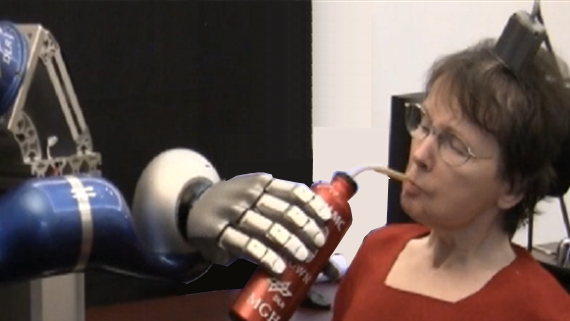
\includegraphics[width=\linewidth]{braingate1}
\caption[Controlling a Robotic Arm through Mental Imagery Alone]{Cathy Hutchinson used the BrainGate system to control a robotic arm with mental imagery alone.  Here she picks up a bottle of water and drinks from it~\cite{Ven12}. Image credit: BrainGate.}
\end{minipage}%
\hfill
\begin{minipage}[t]{.45\textwidth}
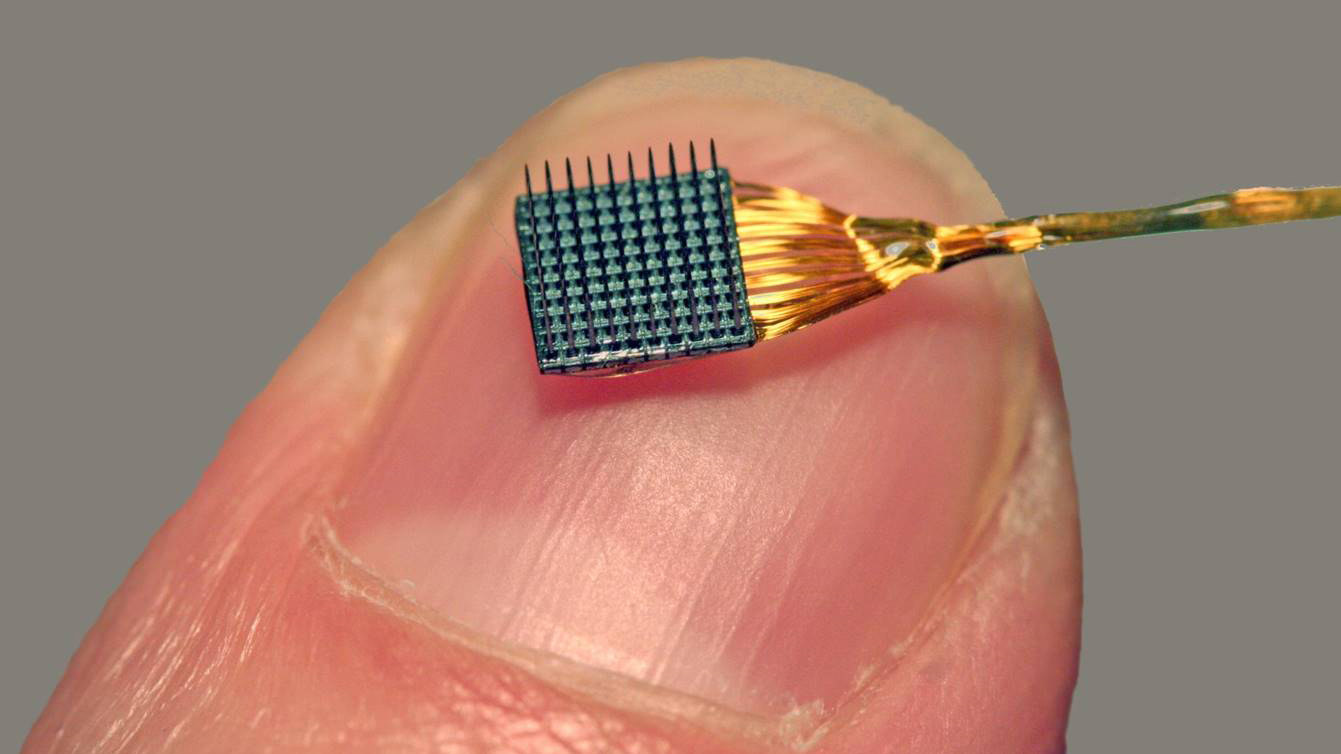
\includegraphics[width=\linewidth]{braingate6}
\caption[The Utah Array]{The BrainGate project uses the Utah Array (Blackrock Microsystems, Salt Lake City, UT) to collect raw neural signals.  Advances in technology have allowed for increasingly more detailed measurements. Image credit: BrainGate.}
\end{minipage}
\end{figure}

%\subsubsection{Filters that are not fast enough}
%Numerical integration methods, such as particle filtering, can be used to approximate the solution to \eqref{e:s2:BF} for essentially any model, but high accuracy approximations may require excessive computation. (Recall that \eqref{e:s2:BF} also involves an implicit integral to compute the constant of proportionality.) There are several methods that use Gaussian approximations to \eqref{e:s2:BF}, making use of the analytic tractability of Gaussians to avoid numerical integration. Laplace approximations, or saddle-point approximations, fit a Gaussian to an integrand by matching the local curvature at the maximum, but they involve an online optimization step that can also be computationally demanding.

\section{Filter Derivation} \label{s:dkf} \index{Discriminative Kalman Filter!derivation}

We derive the DKF under a simplified model for the latent states and discuss generalizations later. Let $\eta_d(z;\mu,\Sigma)$ denote the $d$-dimensional multivariate Gaussian distribution with mean vector $\mu\in\RR^{d\times 1}$ and covariance matrix $\Sigma\in\SS_d$ evaluated at $z\in\RR^{d\times 1}$, where $\SS_d$ denotes the set of $d\!\times\!d$ positive definite (symmetric) matrices.
Assume that the latent states are a stationary, Gaussian, vector autoregressive model of order 1, namely, for $A\in\RR^{d\times d}$ and $S,\Gamma\in\SS_d$,   
\begin{subequations} \label{e:s2:Zmodel}
\begin{align}
 p(z_0) & = \eta_d(z_0;0,S), \label{e:s2:Z} \\ 
 p(z_t|z_{t-1}) & = \eta_d(z_t;Az_{t-1},\Gamma), 
\end{align}
\end{subequations}
for $t=1,2,\dotsc$, where $S=ASA^\tr+\Gamma$, so that the process is stationary. \Eqref{e:s2:Zmodel} is the model for the latent states that underlies the stationary Kalman filter. 

The observations take values in an abstract space ${\cal{X}}$. The observation model $p(x_t|z_t)$ is assumed to not vary with $t$, so that the joint $(Z_t,X_t)$ process is stationary, but it is otherwise arbitrary. It can be non-Gaussian, multimodal, discrete, etc. For instance, in neural decoding, the observations are often vectors of counts of neural spiking events (binned action potentials), which might be restricted to small integers, or even binary-valued. 

The DKF is based on a Gaussian approximation for $p(z_t|x_t)$, namely,
\begin{equation} 
\label{e:s2:DKF-X:deriv} p(z_t|x_t) \approx \eta_d(z_t;f(x_t),Q(x_t)) ,
\end{equation}
where $f:{\cal{X}}\to\RR^d$ and $Q:{\cal{X}}\to\SS_d$. Note that \eqref{e:s2:DKF-X:deriv} is not an approximation of the observation model, but rather of the conditional density of the latent state given the observations at a single time step. When the dimensionality of the observation space (${\cal{X}}$) is large relative to the dimensionality of the state space ($\RR^d$), the Bernstein--von Mises theorem states that there exists $f$ and $Q$ such that this approximation will be accurate, requiring only mild regularity conditions on the observation model $p(x_t|z_t)$ ~\cite[see Section~\ref{s:BVM} and][]{vdV98}. In this paper, we take $f$ and $Q$ to be the conditional mean and covariance of $Z_t$ given $X_t$, namely,
\begin{equation} \label{e:s2:fQ:deriv} f(x)=\Exp(Z_t|X_t=x), \quad Q(x)=\var(Z_t|X_t=x) , \end{equation}
where $\Exp$ and $\var$ denote expected value and variance/covariance, respectively.

To make use of \eqref{e:s2:DKF-X:deriv} for approximating \eqref{e:s2:BF}, we first rewrite \eqref{e:s2:BFb} in terms of $p(z_t|x_t)$, namely
\begin{equation} \label{e:s2:BF2}
p(z_t|x_{1:t}) = \frac{p(z_t|x_t)p(z_t|x_{1:t-1})/p(z_t)}{\int p(z_t|x_t) p(z_t|x_{1:t-1})/p(z_t) \; dz_t} . 
\end{equation}
We then substitute the latent state model in \eqref{e:s2:Zmodel} and the DKF approximation in \eqref{e:s2:DKF-X} into the filtering equations in \eqrefs{e:s2:BFa} and \eqrefMT{e:s2:BF2}, and absorb terms not depending on $z_t$ into a normalizing constant $\kappa$ to obtain
\begin{equation} \label{e:s2:BF2-DKF}
p(z_t|x_{1:t}) \approx \kappa(x_{1:t})\frac{\eta_d(z_t;f(x_t),Q(x_t))}{\eta_d(z_t;0,S)} \cdot \textstyle \int \eta_d(z_t;Az_{t-1},\Gamma) p(z_{t-1}|x_{1:t-1}) \; dz_{t-1} .
\end{equation}
If $p(z_{t-1}|x_{1:t-1})$ is approximately Gaussian, which it is for the base case of $t=1$ from \eqref{e:s2:Z}, then all of the terms on the right side of \eqref{e:s2:BF2-DKF} are approximately Gaussian. If these approximations are exact, we find that the right side of \eqref{e:s2:BF2-DKF} is again Gaussian, giving a Gaussian approximation for $p(z_t|x_{1:t})$. 

Let 
\begin{equation}\label{e:s2:DKp} p(z_t|x_{1:t}) \approx \eta_d(z_t;\mu_t(x_{1:t}),\Sigma_t(x_{1:t})) , \end{equation}
be the Gaussian approximation of $p(z_t|x_{1:t})$ obtained from successively applying the approximation in \eqref{e:s2:BF2-DKF}. Defining $\mu_0=0$ and $\Sigma_0=S$, we can sequentially compute $\mu_t=\mu_t(x_{1:t})\in\RR^{d\times 1}$ and $\Sigma_t=\Sigma_t(x_{1:t})\in\SS_d$ via
\begin{equation} 
\label{e:s2:DKF} 
\boxed{
\begin{aligned}  
M_{t-1} &= A\Sigma_{t-1}A^\tr+\Gamma , \\
\Sigma_t & = (Q(x_t)^{-1}+M_{t-1}^{-1}-S^{-1})^{-1} ,  \\
\mu_t & = \Sigma_t(Q(x_t)^{-1}f(x_t) + M_{t-1}^{-1}A\mu_{t-1}) .
\end{aligned} 
}
\end{equation}
The function $Q$ needs to be defined so that $\Sigma_t$ exists and is a proper covariance matrix.  A sufficient condition that is easy to enforce in practice\footnote{\label{fn:kludge}For our experiments below, if $Q(x_t)^{-1}-S^{-1}\not\in\mathbb{S}_d$ for some $x_t$, we set $S^{-1}=0$ in \eqref{e:s2:DKF}, i.e., we use the robust DKF algorithm for that time step (Section~\ref{s:robust}). This occurs only rarely in practice, as expected from the Bernstein--von Mises Theorem (see Section~\ref{s:BVM}). Even without this result, the Law of Total Variance implies that $\mathbb{E}(S-Q(X_t)) = \var(Z_t) - \mathbb{E}(\var(Z_t|X_t)) = \var(\mathbb{E}(Z_t|X_t))\in\mathbb{S}_d$.} is $Q(\cdot)^{-1}-S^{-1}\in\mathbb{S}_d$.

The DKF is encapsulated in \eqref{e:s2:DKF}. The explicit computations in \eqref{e:s2:DKF} are simple and at least as fast as the Kalman filter. The power of the DKF, along with potential computational difficulties, comes from evaluating $f$ and $Q$. If $f$ is linear and $Q$ is constant, then the DKF is equivalent to the Kalman filter. More general $f$ and $Q$ allow the filter to depend nonlinearly on the observations, improving performance in many cases. If $f$ and $Q$ can be quickly evaluated and the dimension $d$ of $Z_t$ is not too large, then the DKF is fast enough for use in real-time applications, such as the BCI deocoding example below.

\section{Learning} \label{s:learning} \index{Discriminative Kalman Filter!learning filter parameters}

The parameters in the DKF are $A$, $\Gamma$, $Q(\cdot)$, and $f(\cdot)$. ($S$ is specified from $A$ and $\Gamma$ using the stationarity assumption.)  For many real-life problems, these parameters are unknown to us and must be learned from supervised training examples $\{(Z_i',X_i')\}_{i=1}^m$ assumed to be sampled from the underlying Bayesian network in~\eqref{f:graphical_model}.  When we learn DKF parameters, either from a known generating model or from supervised samples, we will denote the learned parameters $\hat A$, $\hat \Gamma$, $\hat Q(\cdot)$, and $\hat f(\cdot)$, respectively.

The model parameters are learned from training data and then fixed and evaluated on testing data. $A$ and $\Gamma$ are the parameters of a well-specified statistical model given by Equations~\ref{e:s2:Z}--\ref{e:s2:ZZ-1}. In the experiments below we learn them from $(Z_{t-1},Z_t)$ pairs using only Equation~\ref{e:s2:ZZ-1}, which reduces to multiple linear regression and is a common approach when learning the parameters of a Kalman filter from fully observed training data~\cite[see, for example,][]{Wu02}. 

The parameters $f$ and $Q$ are more unusual, since they are not uniquely defined by the model, but are introduced via a Gaussian approximation in Equation~\ref{e:s2:DKF-X}.  In cases where the model is known, it may be possible to directly calculate $f$ and $Q$ using \eqref{e:s2:fQ:deriv}.  When the model is not known, $f$ and $Q$ can be learned from a supervised training set.  One possibility is to first learn $p(z_t|x_t)$, either directly or by learning the observation model $p(x_t|z_t)$ and using Bayes' rule, and then derive suitable functions $\hat f$ and $\hat Q$. An alternative approach, and the one we focus on here, is to learn $f$ and $Q$ directly from training data by assuming that Equation~\ref{e:s2:DKF-X} holds exactly, so that $\hat f$ and $\hat Q$ are the conditional mean and covariance of $Z_t$ given $X_t$, namely,
\begin{equation} \label{e:s2:fQ:l} \hat f(x)=\Exp(Z_t|X_t=x), \quad \quad \quad \hat Q(x)=\var(Z_t|X_t=x) , \end{equation}
where $\Exp$ and $\var$ denote expected value and variance/covariance, respectively. The Bernstein--von Mises Theorem holds with this choice of $\hat f$ and $\hat Q$ under some additional mild regularity conditions~\cite{vdV98}. Using Equation~\ref{e:s2:fQ:l}, we learn $f$ and $Q$ from $(Z_t,X_t)$ pairs ignoring the overall temporal structure of the data, which reduces to a standard nonlinear regression problem with normal errors and heteroscedastic variance. The conditional mean $\hat f$ can be learned using any number of off-the-shelf regression tools and then, for instance, $\hat Q$ can be learned from the residuals, ideally, using a held-out portion of the training data. We think that the ability to easily incorporate off-the-shelf discriminative learning tools into a closed-form filtering equation is one of the most exciting and useful aspects of this approach.

In the experiments below, we compare three different nonlinear methods for learning $f$: Nadaraya-Watson (NW) kernel regression, neural network (NN) regression, and Gaussian process (GP) regression.  In all cases, we start with a training set $\{(Z_i',X_i')\}_{i=1}^m$ and form an estimate for $\mathbb{E}[Z|X=x]$.  While we have found that these methods work well with the DKF framework, one could readily use any arbitrary regression model with normal errors.  Depending on the problem domain and the how the observations are generated, one might also consider random forest models, k-nearest neighbors, support vector regression, or even a simple linear regression model using some nonlinear transform of the observed data.

\subsection{Nadaraya-Watson Kernel Regression} \label{s:NW_deriv}  \index{Nadaraya-Watson kernel regression} 
The well-known Nadaraya-Watson kernel regression estimator~\cite{Nad64, Wat64}
\begin{equation} \label{e:s2:NW_f}
\hat f(x) =  \frac{\sum_{i=1}^m Z_i' \kappa_X(x,X_i')}{ \sum_{i=1}^m \kappa_X(x,X_i')}
\end{equation}
where $\kappa_X(\cdot,\cdot)$ is taken to be a Gaussian kernel.  Our implementations of Nadaraya-Watson in the DKF used $\hat f$ as described in \eqref{e:s2:NW_f}.  Bandwidth selection was performed by minimizing leave-one-out MSE on the training set.

\subsection{Neural Network Regression} \label{s:nn} \index{neural networks!for nonlinear regression} 

We can learn $f:\RR^n\to \RR^d$ as a neural network (NN). With mean squared error (MSE) as an objective function, we optimize parameters over the training set.  Typically, optimization continues until performance stops improving on a validation subset (to prevent overfitting), but instead we use Bayesian regularization to ensure network generalizability~\cite{Mac92,For97}.

We implemented all feedforward neural networks with Matlab's Neural Network Toolbox R2017b.  Our implementation consisted of a single hidden layer of tansig neurons trained via Levenberg-Marquardt optimization~\cite{Lev44,Mar63,Hag94} with Bayesian regularization. 

\subsection{Gaussian Process Regression} \label{s:GP} \index{Gaussian process regression} 

Gaussian process (GP) regression~\cite{Ras06} is another popular method for nonlinear regression. The idea is to put a prior distribution on the function $f$ and approximate $f$ with its posterior mean given training data. We will first briefly describe the case $d=1$. We form an $m\times n$-dimensional matrix $X'$ by concatenating the $1\times n$-dimensional vectors $X_i'$ and a $m\times d$-dimensional matrix $Z'$ by concatening the vectors $Z_i'$.  We assume that $p(z_i'|x_i', f)=\eta(z_i'; f(x_i'),\sigma^2)$, where $f$ is sampled from a mean-zero GP with covariance kernel $K(\cdot,\cdot)$. Under this model,
\begin{equation} \label{e:s2:GPf}  
\hat f(x) 
= \Exp(f(x)|Z',X')
= K(x,X')(K(X',X')+\sigma^2 I_m)^{-1} Z',
\end{equation}
where $K(x,X')$ denotes the ${1\!\times\! m}$ vector with $i$th entry $K(x,X_i')$, where $K(X',X')$ denotes the ${m\!\times\! m}$ matrix with $ij$th entry $K(X'_i,X'_j)$, where $Z'$ is a column vector, and where $I_m$ is the ${m\!\times\! m}$ identity matrix. The noise variance $\sigma^2$ and any parameters controlling the kernel shape are hyperparameters. For our examples, we used the radial basis function kernel with two parameters: length scale and maximum covariance.  These hyperparameters were selected via maximum likelihood.  For $d > 1$, we repeated this process for each dimension to separately learn the coordinates of $f$.  

All GP training was performed using the publicly available GPML package~\cite{Ras10}.

\subsection{Learning $Q(\cdot)$} In all cases, we learned the function $Q$ as follows.  We consider the random variable $R_t=Z_t-f(X_t)$ and want to learn
\[ \hat Q(x) = \Exp(R_tR_t^\tr|X_t=x) . \]
Written in this way, we see that $\hat Q(x)$ is a conditional expectation and can in principle be learned with regression from $(\text{vec}(R_tR_t^\tr),X_t)$ pairs, where the vectorization of a matrix $\text{vec}(M)$ simply concatenates the columns into a vector. Since $R_t$ is not observable (because $f$ is unknown), we instead approximate $R_t$ using the learned $f$.   Given a  training set $\{(Z_i'',X_i'')\}_{i=1}^m$ distinct from the one used to learn the function $f$, we define the residuals $\hat R_i=Z_i''-\hat f(X_i'')$, and then learn $Q$ using NW regression on the $\hat R_i$'s of the training data.  Because the NW estimator is a positive linear combination of valid covariance matrices, it will return a valid covariance matrix $Q(x)$ for any $x$.  To avoid overfitting, particularly when $f$ is learned with NW regression, it is helpful to learn $f$ and $Q$ on distinct subsets of the training data.   For the macaque example, the training data was randomly partitioned at a ratio of $70\%-30\%$ into subsets: the first was used to learn $f$ and the second was used to learn $Q$.

\section{Approximation Accuracy} 

\subsection{Bernstein--von Mises theorem} \label{s:BVM} \index{Bernstein--von Mises theorem} 

Let the observation space be ${\cal{X}}=\RR^n$. As $n$ grows, the Bernstein--von Mises (BvM) theorem guarantees under mild assumptions that the conditional distribution of $Z_t|X_t$ is asymptotically normal in total variation distance and concentrates at $Z_t$~\cite{vdV98}. This asymptotic normality result is the main rationale for our key approximation expressed in \eqref{e:s2:DKF-X}. The BvM theorem is usually stated in the context of Bayesian estimation. To apply it in our context, we equate $Z_t$ with the parameter and $X_t$ with the data, so that $p(z_t|x_t)$ becomes the posterior distribution of the parameter. Then we consider the situation where the dimension $n$ of $x_t$ grows, meaning that we are observing growing amounts of data associated with the parameter $Z_t$. 

One concern is that \eqref{e:s2:BF2} will amplify approximation errors. Along these lines, we prove the following result that holds whenever the BvM theorem is applicable for \eqref{e:s2:DKF-X}:
\begin{thm}
Under mild assumptions, the total variation between the DKF approximation for $p(z_t|x_{1:t})$ and the true distribution converges in probability to zero as $n\to\infty$.
\end{thm}
This result is stated formally and proven in the appendix.  We interpret the theorem to mean that under most conditions, as the dimensionality of the observations increases, the approximation error of the DKF tends to zero.

The proof is elementary, but involves several subtleties that arise because of the $p(z_t)$ term in the denominator of \eqref{e:s2:BF2}. This term can amplify approximation errors in the tails of $p(z_t|x_t)$, which are not uniformly controlled by the asymptotic normality results in the BvM theorem. To remedy this, our proof also uses the concentration results in the BvM theorem to control pathological behaviors in the tails. As an intermediate step, we prove that the theorem above still holds when the $p(z_t)$ term is omitted from the denominator of \eqref{e:s2:BF2}.

\subsection{Robust DKF} \label{s:robust} \index{Discriminative Kalman Filter!robust reformulation}

Omitting the $p(z_t)$ from the denominator of \eqref{e:s2:BF2} is also helpful for making the DKF robust to violations of the modeling assumptions and to errors introduced when $f$ and $Q$ are learned from training data. Repeating the original derivation, but without this denominator term gives the following filtering algorithm, that we call the {\em robust DKF}. 
Defining $\mu_1(x_1)=f(x_1)$ and $\Sigma_1(x_1)=Q(x_1)$, we sequentially compute $\mu_t$ and $\Sigma_t$ for $t\geq 2$ via
\begin{equation} 
\label{e:s2:rDKF} 
\boxed{
\begin{aligned}  
M_{t-1} &= A\Sigma_{t-1}A^\tr+\Gamma , \\
\Sigma_t & = (Q(x_t)^{-1}+M_{t-1}^{-1})^{-1} ,  \\
\mu_t & = \Sigma_t(Q(x_t)^{-1}f(x_t) + M_{t-1}^{-1}A\mu_{t-1}) .
\end{aligned} 
}
\end{equation}
Justification for the robust DKF comes from our theoretical results above showing that the robust DKF accurately approximates the true $p(z_t|x_{1:t})$ in total variation distance as $n$ increases. We routinely find that the robust DKF outperforms the DKF on real-data examples, but not on simulated examples that closely match the DKF assumptions.   

\section{More on the Function $Q(\cdot)$}
For random variables $Z\sim\N_d(0,S)$ and $X\in\RR^m$, suppose there exist functions ${g:\RR^m\to\RR^d}$ and ${R:\RR^m\to\SS_d}$ such that
\[
p(x|z) = \eta_d(g(x);z,R(x)),
\]
where $\eta_d(y;\mu,\Sigma)$ denotes the $d$-dimensional Gaussian density with mean $\mu\in\RR^d$ and covariance $\Sigma\in\SS_d$ evaluated at $y\in\RR^d$.  \emph{The issue is that there may not exist many interesting examples of such functions that yield a proper conditional density for $X|Z=z$ for all $z$.}  Then
\begin{align*}
p(x,z) 
&= p(x|z)\:p(z) \\
&= \eta_d(z;g(x),R(x))\: \eta_d(z;0,S) \\
&= \eta_d(g(x);0,R(x)+S)\: \eta_d(z;\tilde f(x),\tilde Q(x)),
\end{align*}
where $\tilde Q(x) = (R(x)^{-1}+S^{-1})^{-1}$ and $\tilde f(x) = \tilde Q(x) R(x)^{-1}g(x)$.  It follows that
\begin{align*}
p(x)
&= \int p(x,z)\; dz \\
&= \eta_d(g(x);0,R(x)+S)\; \int \eta_d(z;\tilde f(x),\tilde Q(x))\; dz \\
&= \eta_d(g(x);0,R(x)+S)
\end{align*}
so we have
\begin{align*}
p(z|x)
&= \frac{p(x,z)}{p(z)} \\
&= \eta_d(z;\tilde f(x),\tilde Q(x)).
\end{align*}
If our functions $\tilde f, \tilde Q$ arrive to us in this way, we can see why it is important to stipulate that $(\tilde Q(x)^{-1}-S^{-1})^{-1}\in\SS_d$ or equivalently that $\tilde Q(x)^{-1}-S^{-1}\in\SS_d$.

\section{Examples}

In this section, we compare filter performance on both artificial models and on real neural data.  Corresponding MATLAB code (and Python code for the LSTM comparison) is freely available online at: \\
\url{github.com/burkh4rt/Discriminative-Kalman-Filter}\\
For timing comparisons, the code was run on a Mid-2012 MacBook Pro laptop with a 2.9 GHz Intel Core i7 processor using MATLAB v. 2017b and Python v. 3.6.4.

\subsection{The Kalman filter: a special case of the DKF}

The stationary Kalman filter observation model is
\[ p(x_t|z_t) = \eta_n(x_t;Hz_t,\Lambda) \]
for observations in ${\cal{X}}=\RR^{n\times 1}$ and for fixed $H\in\RR^{n\times d}$ and $\Lambda\in\SS_n$. Defining $f$ and $Q$ via \eqref{e:s2:fQ:l} gives
\[ f(x) = (S^{-1} + H^\intercal \Lambda^{-1} H)^{-1} H^\intercal \Lambda^{-1} x\]
and
\[ Q(x) \equiv  (S^{-1} + H^\intercal \Lambda^{-1} H)^{-1}. \]
It is straightforward to verify that the DKF in \eqref{e:s2:DKF} is exactly the well-known Kalman filter recursion. Hence, the DKF computes the exact posterior $p(z_t|x_{1:t})$ in this special case.

\subsection{Kalman observation mixtures} \label{s:kalman_mix}

In this section, we consider a family of models for which the Kalman, EKF, and UKF can perform arbitrarily poorly.  Consider the observation model
\[ p(x_t|z_t) = \textstyle \sum_{\ell=1}^L \pi_\ell \eta_n(x_t;H_\ell z_t,\Lambda_\ell) \]
for a probability vector $\pi=\pi_{1:L}$. This a probabilistic mixture of Kalman observation models, one type of switching state space model~\cite[see][]{Shu91,Gha00}
%They have been used in neuroscience for online spike sorting~\cite{Cal11}.
At each time step, one of $L$ possible Kalman observation models is randomly and independently selected according to $\pi$ and then used to generate the observation. Defining $f$ and $Q$ via \eqref{e:s2:fQ:l} gives 
\[ f(x) = \frac{\sum_{\ell=1}^L w_\ell(x) V_\ell x}{\sum_\ell w_\ell(x)}\]
and
\[ Q(x) =  \frac{\sum_{\ell=1}^L w_\ell(x)  (D_\ell + V_\ell x(V_\ell x)^\intercal)}{\sum_{\ell=1}^L w_\ell(x)} - f(x)f(x)^\intercal, \]
where $D_\ell=(H_\ell^\intercal \Lambda_\ell^{-1} H_\ell+ S^{-1})^{-1}$,  $V_\ell= D_\ell H_\ell^\intercal \Lambda_\ell^{-1}$, $G_\ell= H_\ell S H_\ell^\intercal+\Lambda_\ell$, and $w_\ell(x)= \pi_\ell \eta_n(x; 0, G_\ell )$.

Define $\bar H=\sum_{\ell=L} \pi_\ell H_\ell$ so that
\begin{equation} \Exp(X_t|Z_t) = \bar H Z_t \label{e:s2:barH}  . \end{equation}
An interesting special case of this model is when $\bar H=0$, so that the mean of $X_t$ given $Z_t$ does not depend on $Z_t$. Information about the states is only found in higher-order moments of the observations. Algorithms that are designed around $\Exp(X_t|Z_t)$, such as the Kalman filter, EKF, and UKF, are not useful when $\bar H=0$, illustrating the important difference between a Gaussian approximation for the observation model and the DKF approximation in \eqref{e:s2:DKF-X}.

Figure~\ref{fig:mdl62_rmse} shows how the DKF compares to a high-accuracy particle filter (PF) in a simple instance of this model with $d=10$ hidden dimensionality, $L=2$ categories, $\pi=(0.5,0.5)$, $\Lambda_1=I_n$, $\Lambda_2=I_n/8$, and $H_2=-H_1$, so that $\bar H=0$. (The entries of $H_1$ were generated as independent normals.) $S$ is the identity matrix and $A=0.91I-0.1$ has off-diagonal elements, so that the coordinates of $Z_t$ are dependent.  $\Gamma$ was chosen so that $S=ASA^\intercal + \Gamma$.  The test set was 10000 time steps long.  

We believe that the PF is a good approximation to the true posterior, which cannot be exactly computed (to our knowledge).  As $n$ increases, the RMSE (root mean square error) performance of the DKF approaches that of the PF, but the DKF is many orders of magnitude faster (see Figure~\ref{fig:mdl62_rtime}) . A PF that is constrained to run as fast as the DKF has worse performance.


\begin{figure}[h!]
\centering
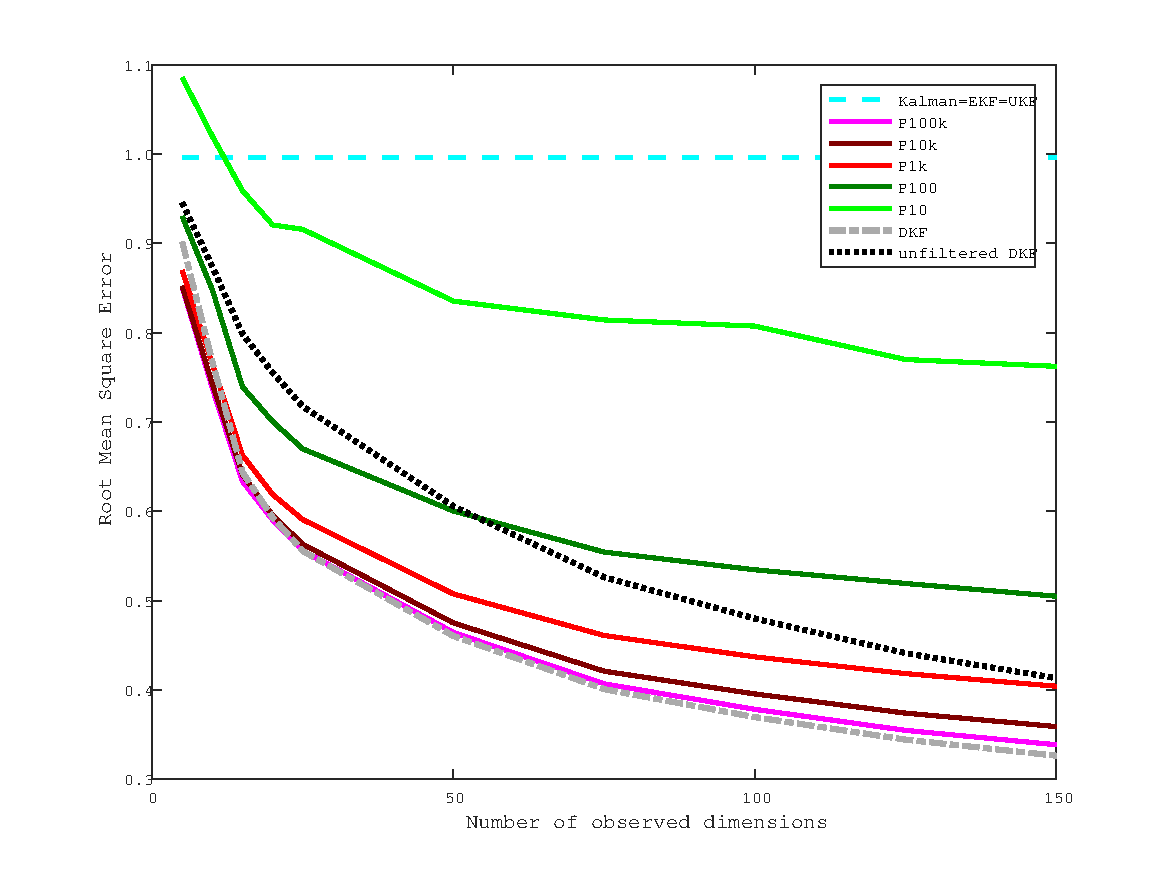
\includegraphics[width=\textwidth]{model62_rmse_plot.pdf}
\caption[A plot of filtering performance (RMSE) on model~\ref{s:kalman_mix} as more dimensions are revealed]{We plot filtering performance (RMSE) on model~\ref{s:kalman_mix} as more dimensions are revealed.}
\label{fig:mdl62_rmse}
\end{figure}

\begin{figure}[h!]
\centering
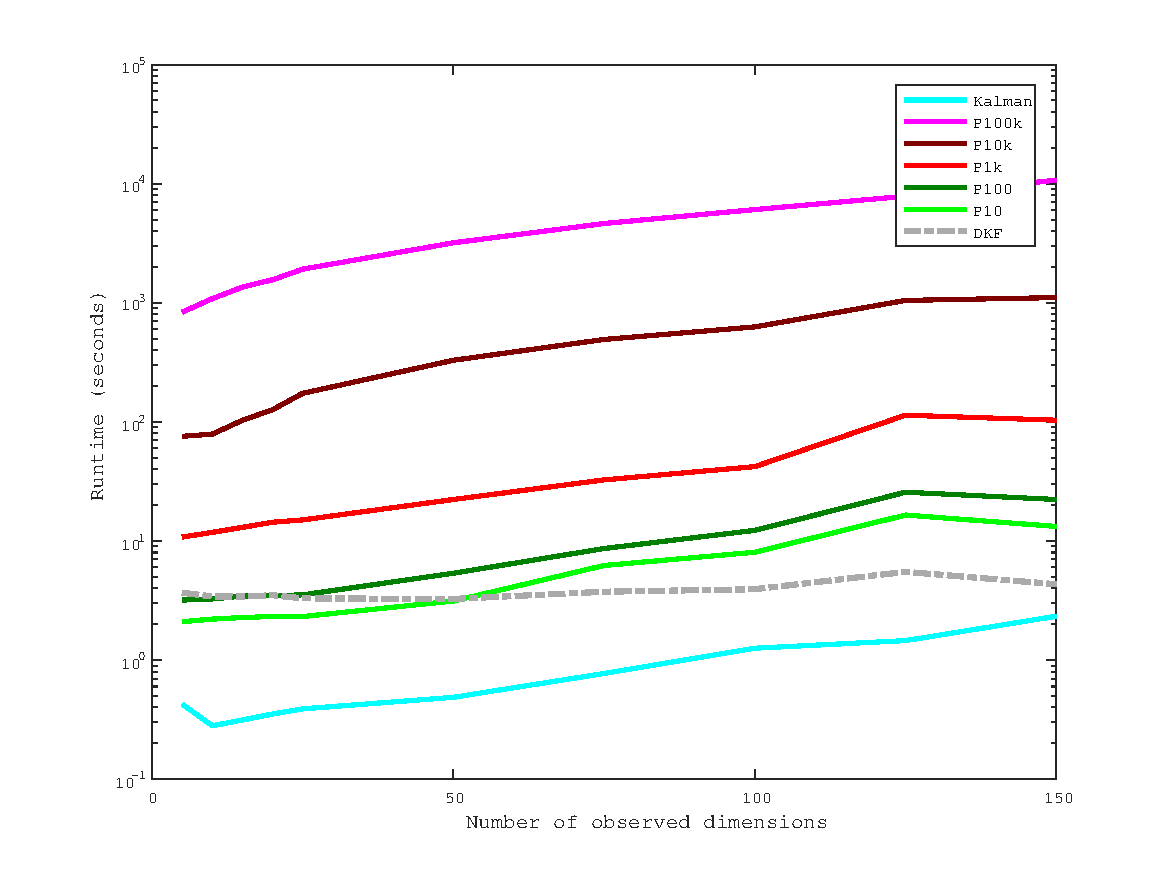
\includegraphics[width=\textwidth]{model62_rtime_plot.pdf}
\caption{Time (in seconds) to calculate all 10000 predictions on model~\ref{s:kalman_mix} as more dimensions are revealed}
\label{fig:mdl62_rtime}
\end{figure}

\subsection{Independent Bernoulli mixtures}
\label{s:iid_bernoulli}

Here we describe a model where observations live in $\{0,1\}^n$. First, consider the case of a single hidden dimension $d=1$. Let $-\infty=c_0<c_1<\dotsb<c_n=\infty$ and define the discrete observation model
\[ p(x_t|z_t) = \textstyle \sum_{\ell=1}^L \pi_\ell \prod_{i=1}^n g_{\ell i}(z_t)^{x_{ti}}(1-g_{\ell i}(z_t))^{1-x_{ti}} \]
where
\[ g_{\ell i}(z) = \textstyle \alpha_{\ell i} + \beta_{\ell i} \mathds{1}_{\{z\ge c_{i-1}\}}, \]
with $\alpha_{\ell i} \geq 0$ and $0 \leq \alpha_{\ell i}+\beta_{\ell i} \leq 1$ for each $1\leq \ell \leq L$ and $ 1\leq i \leq n$.  This is a probabilistic mixture of independent Bernoulli observation models. At each time step $t$, one of $L$ possible models is randomly selected and then used to generate $X_t$. If the $\ell$th model is selected, then the observations are generated as independent Bernoulli's with $\Prob(X_{ti}=1|Z_t)=g_{\ell i}(Z_t)$. In this case, if $\beta_{\ell i} > 0$, then $X_{ti}$ will be one more frequently when $Z_t\ge c_{i-1}$, and vice-versa for $\beta_{\ell i} < 0$.    Define
\[\gamma_{i,\ell}(x) = \pi_\ell \big( \textstyle \prod_{j\ge i} (\alpha_{\ell j} + \beta_{\ell j} )^{x_j}(1-\alpha_{\ell j} - \beta_{\ell j} )^{1-x_j} \big) \big(\textstyle \prod_{j< i} (\alpha_{\ell j} )^{x_j}(1-\alpha_{\ell j})^{1-x_j}\big) \]
so that
\[
p(x_t|z_t) = \textstyle \sum_{\ell=1}^L \gamma_{i,\ell}(x_t)
\]
for $z_t$ in $C_i=[c_{i-1},c_i)$. As the $C_i$ partition $\RR$, for any measurable function $M:\RR\rightarrow\RR$ we can rewrite the following integral as a sum
\begin{align*}
\textstyle \int M(z_t) p(x_t|z_t) p(z_t) dz_t
&=\textstyle \sum_{i=1}^n \int_{C_i} M(z_t) p(x_t|z_t) p(z_t) dz_t \\
&=\textstyle \sum_{i=1}^n  \big(\int_{C_i} M(z_t) p(z_t) dz_t\big) \big(\sum_{\ell=1}^L   \gamma_{i,\ell}(x_t)\big).
\end{align*}
The functions $f$ and $Q$ from \eqref{e:s2:fQ:l} can then be expressed as
\[
f(x) = \frac{\sum_{i=1}^n  \big(\int_{C_i} z p(z) dz\big) \big(\sum_{\ell=1}^L   \gamma_{i,\ell}(x)\big)}{\sum_{i=1}^n  \big(\int_{C_i} p(z) dz\big) \big(\sum_{\ell=1}^L   \gamma_{i,\ell}(x)\big)}
\]
and
\[Q(x) = \frac{\sum_{i=1}^n  \big(\int_{C_i} zz^\intercal p(z) dz\big) \big(\sum_{\ell=1}^L   \gamma_{i,\ell}(x)\big)}{\sum_{i=1}^n  \big(\int_{C_i} p(z) dz\big) \big(\sum_{\ell=1}^L   \gamma_{i,\ell}(x)\big)}  - f(x) (f(x))^\intercal.\]

Note that the above integrals can be re-written in terms of the normal cdf and fully pre-computed before filtering starts. %$\Phi(z) = \Prob(Z_t\leq z)$:

% \begin{align*}
% \int_{C_i} p(z_t) dz_t &= \Phi(c_i) - \Phi(c_{i-1}) \\
% \int_{C_i} z_t p(z_t) dz_t &= (e^{-c_{i-1}^2/2}-e^{-c_i^2/2})/\sqrt{2\pi}  \\
% \int_{C_i} z_t^2 p(z_t) dz_t &= (c_{i-1}e^{-c_{i-1}^2/2}-c_ie^{-c_i^2/2})/\sqrt{2\pi} + \Phi(c_i) - \Phi(c_{i-1})
% \end{align*}

Define $\bar g_i=\sum_\ell g_{\ell i}$, so that
\[ \Exp(X_{ti}|Z_t=z) = \Prob(X_{ti}=1|Z_t=z) = \bar g_i(z) . \]
An interesting special case of this model is when $\bar g_i$ is constant for each $i$, so that the individual components of $X_t$ carry no information about $Z_t$. The vector $X_t$ is needed for predicting $Z_t$. As in the previous section, filtering methods like the Kalman filter, EKF, and UKF are not useful when $\bar g_i$ is constant. 

We can add observed dimensions to the model by refining the partition $c_0<c_1<\dotsb<c_n$.  This yields a model of the same form where the additional dimensions in $X_t$ provide more information about $Z_t$.

Figure \ref{fig:mdl43_rmse} shows how the DKF compares to a high-accuracy particle filter in a simple instance of this model with $d=3$, where each dimension of $Z_t$ was generated independently under an independent choice of model $\ell$ and the $X_t$ values for each dimension were concatenated.  The single-dimensional model took $L=2$, $\pi=(0.5,0.5)$, $\alpha_{1 i}=0.001$, $\beta_{1 i}=0.998$, $\alpha_{2 i}=1-\alpha_{1 i}$, $\beta_{2 i}=-\beta_{1 i}$, so that $g_{2 i}(z)=1-g_{1 i}(z)$ and $\bar g_i(z)\equiv 0.5$, for all $i$. The partition $-\infty=c_0<c_1<\dotsb<c_n=\infty$ was chosen so that $Z_t$ was equally likely to fall into any of the intervals, i.e. to make $\Prob(c_{i-1}\leq Z_t < c_i) = 1/n$ for all $i$.  $S$ is the identity matrix and $A=0.3I+0.2$ has off-diagonal elements, so that the coordinates of $Z_t$ are dependent.  $\Gamma$ was chosen so that $S=ASA^\intercal + \Gamma$. 

This example emphasizes that the DKF can be used with highly non-Gaussian observation models, because its Gaussian approximation is in the state space, not the observation space.  Again, PF's that run faster than the DKF perform significantly worse as the dimensionality of observations grows (see Figure~\ref{fig:mdl43_rtime}).

\begin{figure}[h!]
\centering
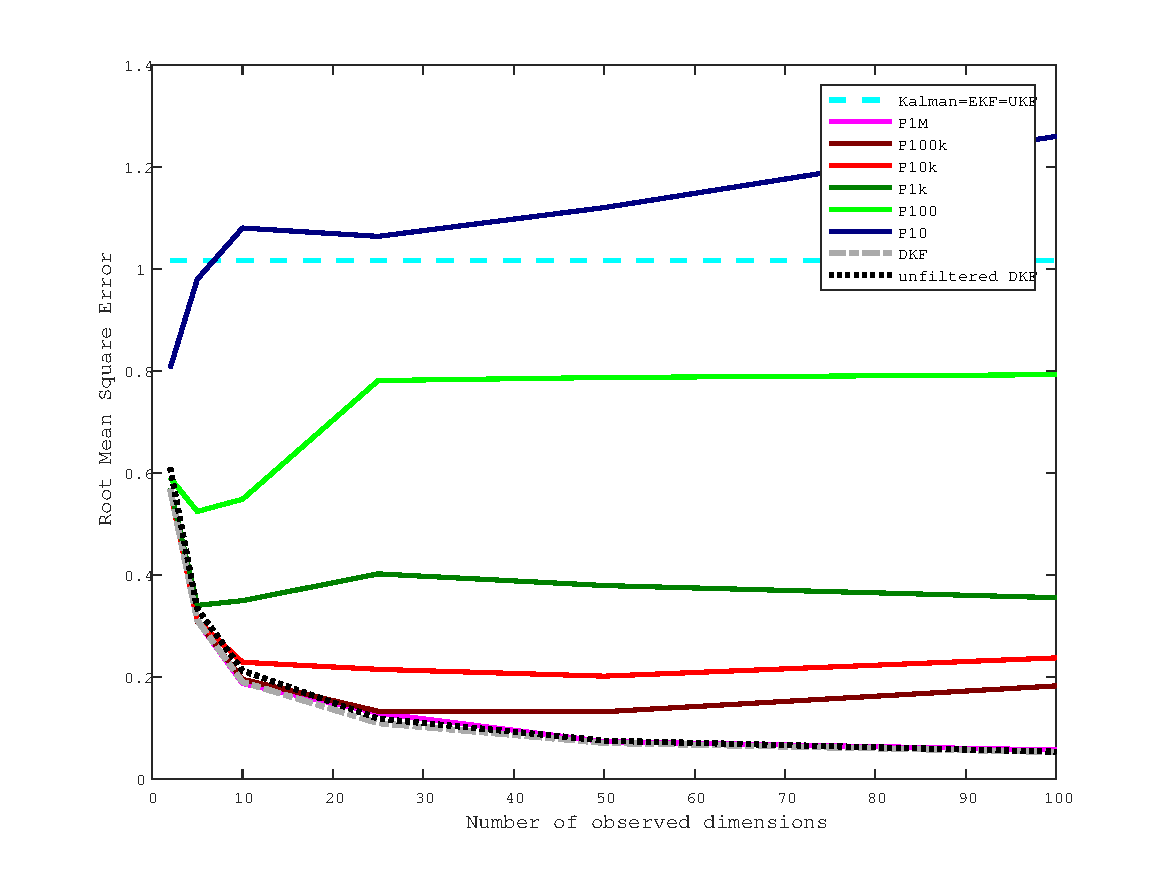
\includegraphics[width=\textwidth]{model63_rmse_plot.pdf}
\caption[A plot of filtering performance (RMSE) on model~\ref{s:iid_bernoulli} as more dimensions are revealed.]{We plot filtering performance (RMSE) on model~\ref{s:iid_bernoulli} as more dimensions are revealed.}
\label{fig:mdl43_rmse}
\end{figure}

\begin{figure}[h!]
\centering
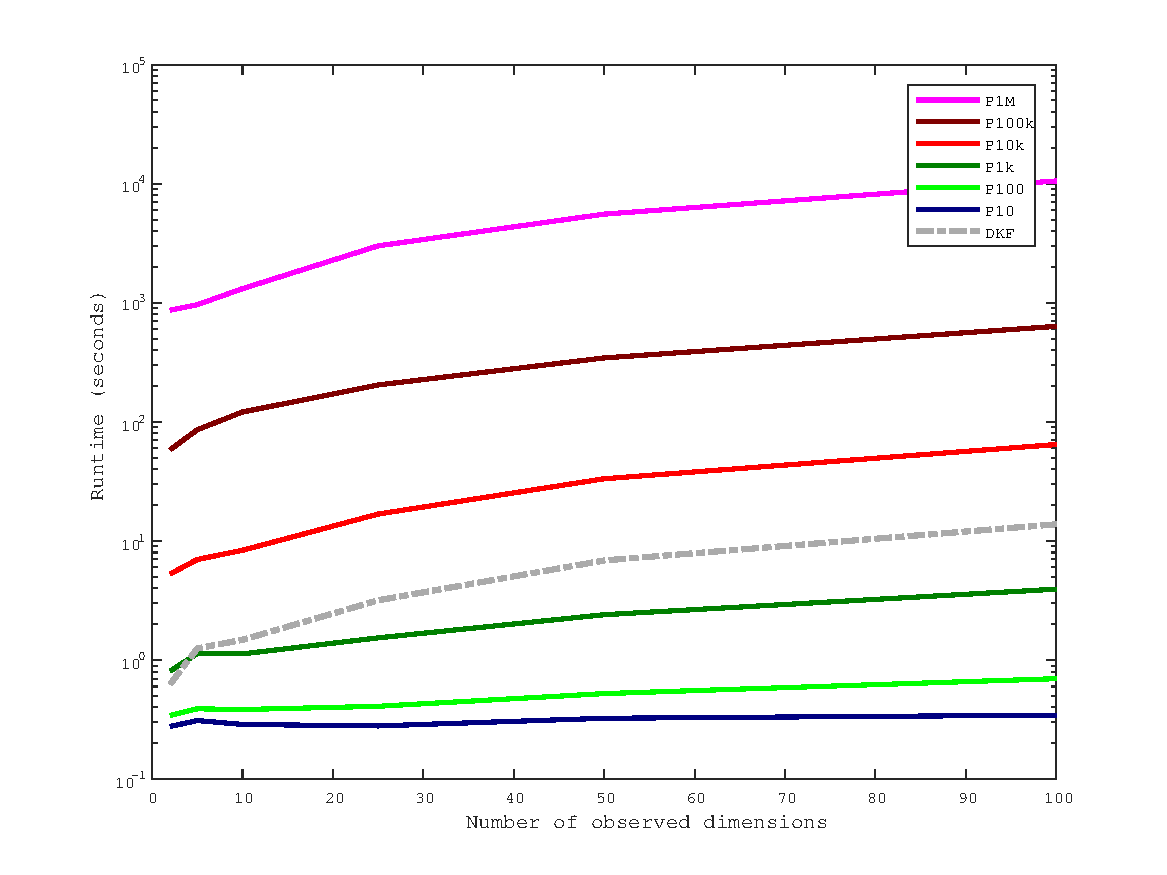
\includegraphics[width=\textwidth]{model63_rtime_plot.pdf}
\caption{Time (in seconds) to calculate all 1000 predictions on model~\ref{s:iid_bernoulli} as more dimensions are revealed}
\label{fig:mdl43_rtime}
\end{figure}

\subsection{Unknown observation model: Macaque reaching task data} \index{neural filtering!in rhesus monkeys}

\textcite{Fli12} implanted a rhesus monkey with a 96-channel microelectrode array (Blackrock Microsystems LLC) over the arm area of its primary motor cortex (M1).  The monkey was trained to move a manipulandum to acquire illuminated targets for a juice reward.  While performing this task, the monkey's neural spikes were recorded with a 128-channel acquisition system (Cerebus, Blackrock Microsystems LLC).  The signal was sampled at 30 kHz, high-pass filtered at 300 Hz, and then manually thresholded and sorted into spikes offline. ~\textcite*{Wal13} continue to make this data publicly available as part of the Database for Reaching Experiments and Models (DREAM).  We took the data from~\textcite{Fli12} and took spike counts over 100ms bins.  The first 10 PCA components of neural data became the observed variable.

Filtering results can be found in Table~\ref{t:monkey_maae}.  We normalize RMSE by dividing it by the root mean square of the observation vector, so that predicting identically zero would yield a normalized RMSE of 1.  We also present mean absolute angular error.  Because cursor speed is often adjustable in BCIs, this may provide a more informative measure of performance.

\subsection{Comparison with a Long Short Term Memory (LSTM) neural network} \index{neural networks!Long Short-Term Memory} 

An LSTM is a stateful recurrent neural network designed to overcome error backflow problems~\cite{Hoc97}.  Such recurrent neural networks have previously been shown to outperform state-of-the-art Kalman-based filters on this primate neural decoding task and so provide a good point of comparison~\cite{Sus12,Sus16}.  While there are many variants on the LSTM architecture, none seem to universally improve on the basic design~\cite{Joz15,Gre16}.

All LSTM trials were conducted with TensorFlow r1.5~\cite{Aba15} in a Python 3.6.4 environment. The LSTM cell used in these trials was built from scratch in TensorFlow following~\cite{Ger00a}.  Dropout was used to prevent overfitting~\cite{Sri14}\index{neural networks!dropout}, but it was only applied to feedforward connections, not recurrent connections~\cite{Pha14, Zar14}.  The recurrent states and outputs at each intermediate timestep were batch-normalized to accommodate internal covariate shift~\cite{Iof15}.  
% Peephole connections between the state and gates~\cite{Ger00b} were used for the artificial data sets only.
Model parameters were initialized via a Xavier-type method~\cite{Glo10} designed to stabilize variance from layer to layer.  Optimization was then performed with Adadelta~\cite{Zei12}, an algorithm designed to improve upon Adagrad~\cite{Duc11} with the explicit goals of decreasing sensitivity to hyperparameters and permitting the learning rate to sometimes increase.

One advantage to the DKF approach is that good model selection requires minimal expert intervention.  The LSTM and variants require manually selecting a neural network architecture.  This is often done by experts through trial and error.  Automating this process remains an area of active research requiring extensive computational resources~\cite{Zop17,Rea17}.  

%%%%%%%%%%%%%%%%%%%%%%%%%%%%%%%%%%%%%%%%%%%%%%%%%
\begin{figure}[h]
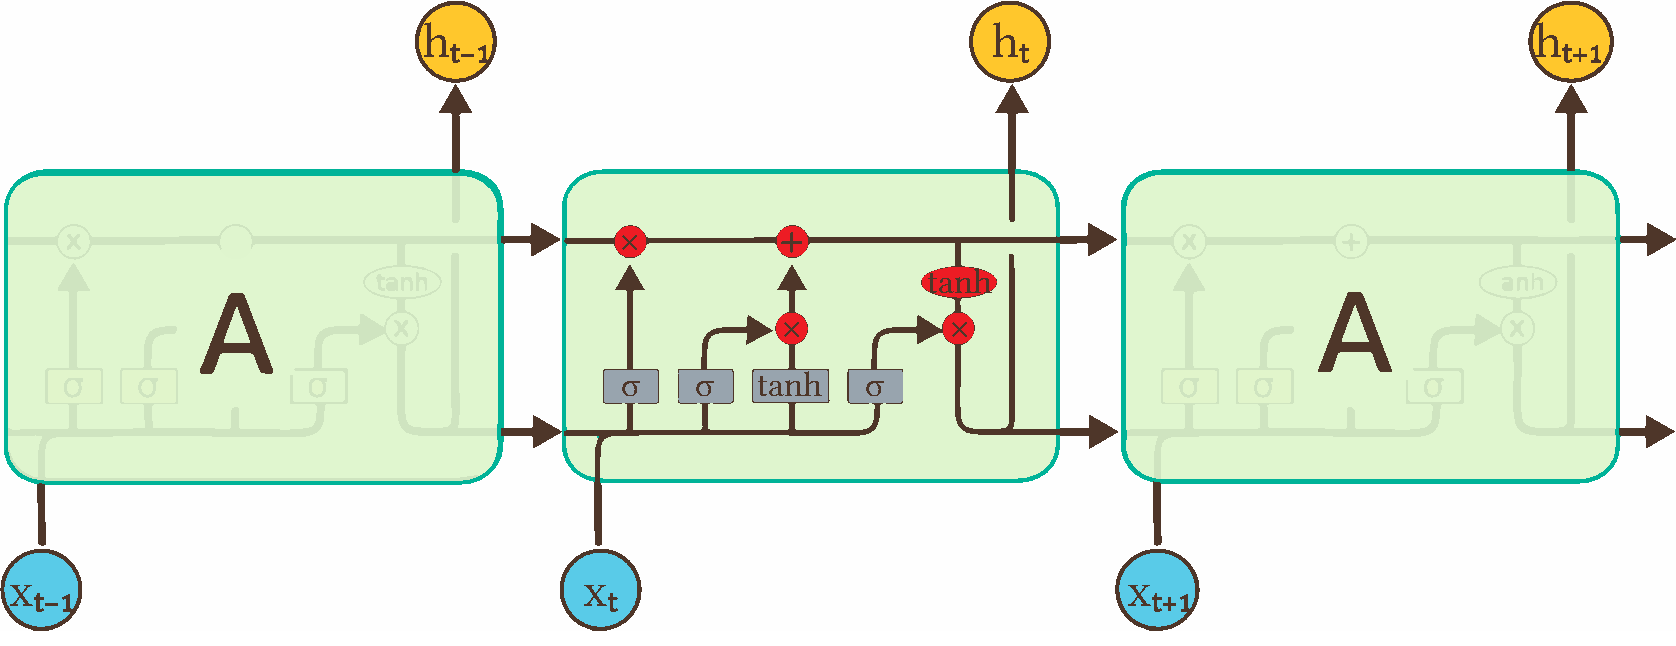
\includegraphics[width=\linewidth]{lstm_chain}
\caption[LSTM schematic]{This diagram gives a schematic representation of an LSTM cell.  Re-used with permission: \textcite{Ola15}.}
\end{figure}


% \begin{table*}[ht]
% \centering
% \caption{\% Change in Normalized RMSE from Kalman baseline on the Flint dataset}
% \label{t:monkey_nrmse}
% \begin{tabular}{|l|llllll|l|} \hline
%        & Trial 1 & Trial 2 & Trial 3 & Trial 4 & Trial 5 & Trial 6 & Avg.  \\ \hline
% Kalman & 0.765   & 0.942   & 0.788   & 0.793   & 0.780   & 0.765   & 0.805 \\ \hline
% DKF-NW & -21\%   & -18\%   & -17\%   & -23\%   & -20\%   & -23\%   & -20\% \\
% DKF-NN & -19\%   & -15\%   & -13\%   & -13\%   & -13\%   & -17\%   & -15\% \\
% DKF-GP & -21\%   & -19\%   & -15\%   & -20\%   & -18\%   & -20\%   & -19\% \\ \hline
% LSTM   & -15\%   & -19\%   & -16\%   & -13\%   & -16\%   & -11\%   & -15\% \\ \hline
% EKF    & 2\%     & 24\%    & 12\%    & 18\%    & 12\%    & 3\%     & 12\%  \\
% UKF    & 2\%     & 31\%    & 18\%    & 18\%    & 15\%    & 6\%     & 15\%  \\ \hline
% \end{tabular}
% \end{table*}

\begin{table*}[ht]
\centering
\caption{\% Change in Mean Absolute Angular Error (Radians) Relative to Kalman}
\label{t:monkey_maae}
\begin{tabular}{|l|llllll|l|}
\hline
              & Trial 1 & Trial 2 & Trial 3 & Trial 4 & Trial 5 & Trial 6 & Avg   \\ \hline
Kalman        & 0.889   & 0.955   & 1.025   & 0.933   & 0.964   & 0.926   & 0.949 \\ \hline
DKF-NW        & -15\%   & -1\%    & -20\%   & -17\%   & -25\%   & -28\%   & -18\% \\
DKF-NN        & -7\%    & -2\%    & -17\%   & -16\%   & -21\%   & -23\%   & -14\% \\
DKF-GP        & -11\%   & 7\%     & -22\%   & -16\%   & -24\%   & -25\%   & -15\% \\ \hline
UKF           & 0\%     & 3\%     & -3\%    & -3\%    & -8\%    & -6\%    & -3\%  \\ 
EKF           & 4\%     & 3\%     & -2\%    & -4\%    & -8\%    & -7\%    & -2\%  \\ \hline
LSTM          & -2\%    & -2\%    & -12\%   & -6\%    & -10\%   & -8\%    & -7\%  \\ \hline
Unfiltered NW & -9\%    & 1\%     & -22\%   & -17\%   & -20\%   & -26\%   & -16\% \\ 
Unfiltered NN & -3\%    & -0\%    & -17\%   & -14\%   & -17\%   & -17\%   & -11\% \\ 
Unfiltered GP & -5\%    & 10\%    & -21\%   & -14\%   & -18\%   & -20\%   & -12\% \\ \hline
\end{tabular}
\end{table*}

\section{Closed-loop decoding in a person with paralysis} \label{s:human_data} \index{neural filtering!in humans} 

\subsection{Participant}

The participant in this study was T9, a 52 year-old right-handed male with paralysis from late stage amyotrophic lateral sclerosis (ALSFRS-score = 7). T9 underwent surgical placement of two 96-channel intracortical silicon microelectrode arrays~\cite{May97} (1.5-mm electrode length, Blackrock Microsystems, Salt Lake City, UT) in the primary motor cortex as previously described~\cite{Kim08, Sim11}.  Data was used from trial (post-implant) days 292 and 293.

\subsection{Signal acquisition}

Raw neural signals for each channel (electrode) were sampled at 30kHz using the NeuroPort System (Blackrock Microsystems, Salt Lake City, UT). Further signal processing and neural decoding were performed using the xPC target real-time operating system (Mathworks, Natick, MA). Raw signals were downsampled to 15kHz for decoding, and de-noised by subtracting an instantaneous common average reference~\cite{Gil15, Jar15} using 40 of the 96 channels on each array with the lowest root-mean-square value (selected based on their baseline activity during a one minute reference block run at the start of each session). The de-noised signal was band-pass filtered between 250 Hz and 5000 Hz using an 8th order non-causal Butterworth filter~\cite{Mas15}. Spike events were triggered by crossing a threshold set at 3.5x the root-mean-square amplitude of each channel, as determined by data from the reference block. The neural features used was the the total power in the band-pass filtered signal~\cite{Jar15, Bra18}. Neural features were binned in 20ms non-overlapping increments for decoding. We used the top 40 features ranked by signal-to-noise-ratio~\cite{Mal15}. 

\subsection{Decoder Calibration}

Decoder calibration was performed using the standard Radial-8 task~\cite{Sim11, Gil15} using custom built software running Matlab (Natick, MA). An LCD monitor was placed 55-60 cm at a comfortable angle and orientation to T9. Targets (size = 2.4 cm, visual angle = $2.5\degree$) were presented sequentially in a pseudo-random order, alternating between one of eight radially distributed targets and a center target (radial target distance from center = 12.1 cm, visual angle = $12.6\degree$). Successful target acquisition required the user to place the cursor (size = 1.5cm, visual angle = 1.6$\degree$) within the target's diameter for 300ms, before a pre-determined timeout of 15 seconds. Target timeouts resulted in the cursor moving directly to the intended target, with immediate presentation of the next target.

Calibration began with two minute of open-loop presentation of a cursor; that is, the cursor moved automatically to pseudorandomly presented targets in a straight path. During this time, T9 was instructed to ``imagine'' or ``attempt'' to move the computer cursor as if he had control of it. After two minutes, initial coefficients were computed for the Gaussian process decoder.  Next, T9 acquired targets for three minutes with 80\% of the component of the decoded vector perpendicular to the vector between the cursor and the target~\cite{Jar13, Vel08}. Coefficients were then recomputed with all of the available data. The Radial-8 task was repeated two more times with the attenuated components at 50\% and 20\%, for a total of 11 minutes of calibration data collected. We collected a total of 3000 datapoints randomly subsampled from the 11 minutes of collected data, using all 192 neural features (96 features per array, two arrays).

\subsection{Performance measurement} \index{Discriminative Kalman Filter!online human neural decoding experiment}

We quantified the performance of the DKF decoder with the mFitts1 task ~\cite{Gil15, Sim11}. A single target was presented on the screen in a pseudorandom location, with one of three pseudorandomly fixed diameters (size = 1.6cm, 3.5cm, and 5.6cm, visual angles 1.7$\degree$, 3.7$\degree$, and 5.8$\degree$). Targets were acquired by having the cursor contact the target for 500ms milliseconds, within a timeout of 10 seconds. 

For the mFitts1 task, the Index of Difficulty for each trial was calculated as follows:
\begin{equation} 
\label{e:s2:Fitts} ID = \log_2\left[ \frac{D}{W} + 1 \right]
\end{equation}
where D is the distance from the cursor's start position to the goal, and W is the sum of the target's diameter and cursor's radius. Hence, $\frac{D}{W}$ reflects a measure of difficulty for acquiring targets. 

\subsection{Results}

\begin{figure}
\centering
\begin{minipage}{.49\linewidth}
  \centering
  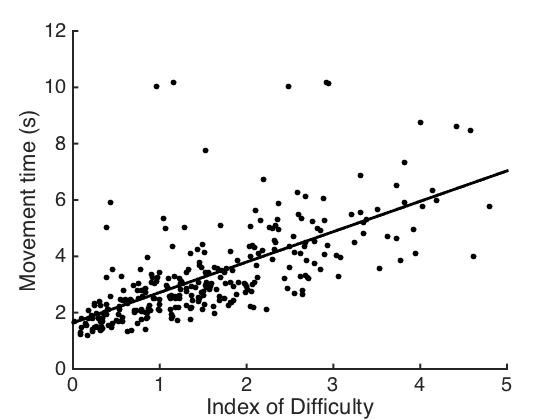
\includegraphics[width=\linewidth]{FittsPlot1.png}
\end{minipage}%
\begin{minipage}{.49\linewidth}
  \centering
  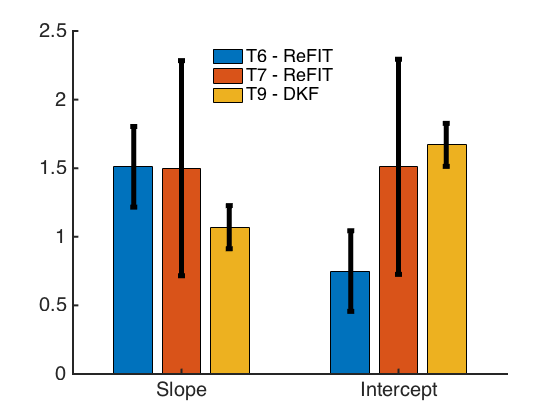
\includegraphics[width=\linewidth]{FittsPlot2.png}
\end{minipage}%
\caption{Fitts plots comparing the DKF to Kalman ReFit}
\label{fig:fitts}
\end{figure}

T9 acquired 98\% of targets presented over two research sessions (N = 299) with the mFitts1 task. The Fitts regression parameters were comparable to the previously described performance using the ReFIT decoder~\cite{Gil15} (Fig.~\ref{fig:fitts}, slope = $1.08 \pm 0.06 p < 1.2 \times 10^{-30}$, intercept = $1.6  \pm 1.3, p < 2.2 \times 10^{-41}$).

\section{Run Time}
As code runtime can vary highly by choice of language and implementation details, we discuss the theoretical time-limiting steps involved for the different filtering methods and describe how these costs grow with model parameters and size of the training set.

\subsection{Training Requirements}
Training the DKF entails learning $f(\cdot)\in\RR^d$ and $Q(\cdot)\in\RR^{d\times d}$ from Equation~\ref{e:s2:DKF-X}.  We consider how training costs grow with the number of training points $m$.  If $f$ is learned with NW, bandwidth can be chosen using rule-of-thumb (free) or with leave-one-out cross validation scaling as $\mathcal{O}(m^2)$. If $f$ is learned as a NN, training costs depend on the training algorithm chosen.  Traditional optimizers include:s2: stochastic gradient descent, scaling with $\mathcal{O}(m)$; scaled conjugate gradient, with $\mathcal{O}(m^2)$; Levenberg--Marquardt, with $\mathcal{O}(m^3)$~\cite{Cas06}.  More recently, Hessian-free approaches have been developed to train NN's on larger data sets~\cite{Sch15}.  Training costs also grow with $d$, depending on choice of architecture.  If $f$ are learned as a GP, training costs scale as $\mathcal{O}(m^3)$.  Sparse approximations to GP's can reduce training requirements to $\mathcal{O}(m\cdot N_S^2)$ where $N_S$ is the size of the sparse GP~\cite{Qui05}.

Fitting a linear model for the KF requires least squares regression, which tends to be fast.  Training an EKF or UKF model entails learning the function $h$  and the noise covariance parameter $\Lambda$ in the measurement model ${p(x_t|z_t) = \eta_m(h(z_t),\Lambda)}$.  If done with a NN, costs depend on the training algorithm chosen (see above).  LSTM optimization uses many of the same methods that work for feedforward NN's~\cite{Sch15}.

\subsection{Prediction Requirements}  
An iteration of the DKF requires computing $f(\cdot)\in\RR^d$ and $Q(\cdot)\in\RR^{d\times d}$ along with a few inversions and multiplications in $\operatorname{Mat}(d\times d)$, where $d$ tends to be small.  If $Q(\cdot)$ is calculated on held-out training data and then fixed, the posterior covariance quickly converges to a limiting value and can itself be fixed, further reducing computational costs. 

The EKF and UKF both tend to be relatively fast, but they specify a very specific form for $p(x_t|z_t)$ and can perform rather poorly when that form is a poor approximation to the true model (for example, they are completely ineffective on the models described in sections~\ref{s:kalman_mix} and~\ref{s:iid_bernoulli}).

Transitioning to more general nonlinear filtering often entails nonparametric methods with costs that scale with $m$.  NW regression also scales $\mathcal{O}(m)$ for evaluating $\hat f$.  NN's scale $\mathcal{O}(1)$ for evaluation.  GP's scale $\mathcal{O}(m)$ for $\hat f$ and their sparse approximations scale $\mathcal{O}(N_S)$ where $N_S$ is the size of the sparse GP~\cite{Qui05}.  Among the non-probabilistic methods, evaluating a neural network scales $\mathcal{O}(1)$ with training size, including the LSTM.

\section{Discussion}

The DKF is a novel approximation scheme that should be a helpful addition to the filtering toolbox. It provides a fast, analytic filtering approximation for models with linear, Gaussian dynamics, but nonlinear, non-Gaussian observations. The approximations underlying the DKF tend to improve as the dimensionality of the observation space increases relative to the dimensionality of the state space. Of existing filtering approximations, the DKF seems most closely related to Laplace approximations, or saddle-point approximations, but there are important differences. Laplace approximations are based on the local curvature of the posterior, whereas the DKF is a global approximation. Laplace approximations also involve an online optimization step that can be computationally demanding. The approximations underlying the DKF are conceptually distinct from those underlying the well-known EKF and UKF, and the methods are useful in different situations.

One potential drawback of the DKF is that it requires the conditional mean and variance of states ($Z_t$) given observations ($X_t$), which are often difficult to compute from the standard generative formulation of a state-space model. If, however, the model must be learned from supervised training data prior to filtering, then off-the-shelf nonlinear and/or nonparametric regression tools can be used to learn the conditional mean and variance directly, avoiding the more complicated task of learning the complete observation model $p(x_t|z_t)$. The benefits of this simplification are amplified in situations where the observation-dimensionality is much higher than the state-dimensionality. Using the DKF in this way appears to be novel within the large literature on learning state space models. Most approaches either learn a fully generative model and invert it for filtering (this includes the of use discriminative methods for training filters derived from generative models~\cite{Abb05,Hes09}), or learn a fully discriminative model that directly predicts states from the sequence of observations. The DKF allows a generative model for the state dynamics to be combined in principled way with a discriminative model for predicting the states from the observations at individual time steps.  We think that the ability to easily incorporate off-the-shelf discriminative learning tools into a closed-form filtering equation is one of the most exciting and useful aspects of this methodology.

Another drawback of the DKF is its restriction to linear, Gaussian state dynamics.  However, it is possible to use the discriminative measurement update approximation 
\begin{equation} \label{eq:discriminative_observation_approx}
p(x_t|z_t) =  p(x_t) \frac{p(z_t|x_t)}{p(z_t)}
\approx \kappa(x_t) \frac{\eta_d(z_t;f(x_t),Q(x_t))}{\eta_d(z_t;0,S)}
\end{equation}
in conjunction with the EKF or UKF method for propagating state dynamics.  In the case that $p(z_t|z_{t-1})$ is nonlinear, it is worth noting that the denominator $\eta_d(z_t;0,S)$ will no longer precisely correspond to $p(z_t)$ but will also be an approximation.  If the Gaussian approximations for $p(z_t|x_t)$ and $p(z_t)$ are learned separately, some care may need to be taken to ensure the resulting approximation to $p(x_t|z_t)$ remains a good one.  In Section~\ref{s:nonlinear_state_ex}, we illustrate an example where using a discriminative observation update with EKF/UKF state updates yields a much better filter than the standard EKF/UKF.  Analogously, within a particle filter, particle weights can be updated using the discriminative approximation in ~\eqref{eq:discriminative_observation_approx}.  This approach may be useful in situations where the observation model must be learned from data.  In future work, we plan to explore this and other approaches that might allow a DKF-style approximation to be incorporated into more general filtering models.

The DKF approximation assumes a Gaussian posterior and is unlikely to work well in problems where it is important to maintain the full shape of a multimodal posterior. In situations with unknown models, however, there may be benefits to combining more accurate methods, like particle filtering, with alternatively-specified filtering equations, as in \eqref{e:s2:BF2}, in order to create general purpose filters that are both more convenient to learn from data and more convenient to use in filtering applications. The DKF is a first step in this direction.

%Other filtering approaches, incorporating non-parametric regression techniques, have been described in the literature. For instance,  the Gaussian process factor analysis (GPFA) method models $p(x_t|z_t)$ as linear plus Gaussian noise, while $p(z_t)$ is modeled by a 0-mean Gaussian process~\cite{Yu09}. Since the latent variables are not observed, both the filter parameters and latent variables are learned by expectation maximization. This method introduces the machinery of Gaussian processes, but maintains a linear relationship between observations and latent variables.

%The GP-BayesFilters uses HMM with the Gaussian process framework~\cite{Ko09}. Both $p(x_t|z_t)$ and $p(z_t|z_{t-1})$ are modeled by Gaussian processes so that a particle filtering or UKF approximation is required.    

\section{Example with Nonlinear State Dynamics} \label{s:nonlinear_state_ex} \index{Discriminative Kalman Filter!adaptation to nonlinear state dynamics}
Consider the state model
\begin{equation} \label{eq:nonlinearstate}
p(z_t|z_{t-1}) = \eta_d(A(\sin(z_{t-1})+z_{t-1}),\Gamma)
\end{equation}
for $A\in \RR^{d\times d}, \Gamma\in \SS_d$ and observation model
\begin{equation}
p(x_t|z_t) 
= \eta_m(h(z_t)+z_t/3,\Lambda)
\end{equation}
where $\Lambda \in \SS_m$ and $h:\RR^d\rightarrow\RR^m$ concatenates the component-wise floor function $\lfloor z_t-a_j\rfloor$ over a set of $m/d$ elements $a_j\in\RR^d$.

The stationary distribution of $Z_t$ is not Gaussian (and cannot be expressed analytically) so we learn $\hat f$ by generating ten thousand samples from the joint distribution of $(X_t,Z_t)$ and learning a NN.  We compute the covariance of the residuals on heldout data and use this fixed value for $\hat Q$.  Finally, $S$ can be approximated well using a Taylor series expansion for sine and the recursion~\eqref{eq:nonlinearstate} or from samples.  This gives us the necessary ingredients for our discriminative approximation 
\begin{equation} \label{eq:dkf-observation-update}
p(x_t|z_t) =  p(x_t) \frac{p(z_t|x_t)}{p(z_t)}
\approx \kappa(x_t) \frac{\eta_d(z_t;f(x_t),Q(x_t))}{\eta_d(z_t;0,S)}
\end{equation}
For this example, we used EKF/UKF approach to move from a Gaussian approximation of $p(z_{t-1}|x_{1:t-1})$ to a Gaussian approximation of $p(z_t|x_{1:t-1})$ and then the DKF approximation in \eqref{eq:dkf-observation-update} to move from a Gaussian approximation of $p(z_t|x_{1:t-1})$ to a Gaussian approximation of $p(z_t|x_{1:t})$.  Additionally, we implemented a SIR particle filter that used the true state dynamics and the DKF approximation~\eqref{eq:dkf-observation-update} for particle re-weighting.  Results over five independent trials are summarized in Table~\ref{t:model9-results}.

\begin{table*}[h]
\centering
\caption{Normalized RMSE for different filtering approaches to Model~\ref{s:nonlinear_state_ex}}
\label{t:model9-results}
\begin{tabular}{|l|lllll|l|}
\hline
                                     & Trial 1 & Trial 2 & Trial 3 & Trial 4 & Trial 5 & Average \\ \hline
Particle Filter                       & 0.327   & 0.318   & 0.331   & 0.335   & 0.335   & 0.329   \\
PF with DKF re-weighting & 0.328   & 0.319   & 0.334   & 0.336   & 0.341   & 0.332   \\ \hline
EKF                                   & 0.414   & 0.392   & 0.414   & 0.424   & 0.430   & 0.415   \\
EKF-state, DKF-observation            & 0.328   & 0.319   & 0.333   & 0.336   & 0.340   & 0.331   \\ \hline
UKF                                   & 0.476   & 0.471   & 0.444   & 0.480   & 0.491   & 0.472   \\
UKF-state, DKF-observation            & 0.327   & 0.318   & 0.332   & 0.336   & 0.339   & 0.331   \\ \hline
Unfiltered                            & 0.352   & 0.341   & 0.355   & 0.362   & 0.355   & 0.353   \\ \hline
\end{tabular}
\end{table*}

The EKF and UKF filters can be implemented exactly for this model, but because $h'(z)=0$ for almost every $z$, both filters perform quite poorly.  This example serves to illustrate how a discriminatively-learned observation model can be successfully incorporated within standard filtering frameworks.


